\section*{Problem 2 - Straight-line path following in the horizontal plane}

\subsection*{Problem 2.1}

Using the kinematics in chapter 2 in book by Fossen \cite{Fossen2011} we have

\begin{align}
    \dot{\eta} &= R(\psi)v \\
    \begin{bmatrix}
    \dot{x} \\
    \dot{y} \\
    \dot{\psi}
    \end{bmatrix} 
    &=
    \begin{bmatrix}
    \cos{\psi} & -\sin{\psi} & 0 \\
    \sin{\psi} & \cos{\psi} & 0 \\
    0 & 0 & 1 \\        
    \end{bmatrix}
    \begin{bmatrix}
    u \\
    v \\
    r
    \end{bmatrix} \\
    \rightarrow 
    \begin{bmatrix}
    \dot{x} \\
    \dot{y}
    \end{bmatrix}
    &=
    \begin{bmatrix}
    u\cos(\psi) - v\sin(\psi) \\
    u\sin(\psi) + v\cos(\psi) 
    \end{bmatrix}
\end{align}

Here we assume that $\theta$ and $\phi$ are small enough so that $\cos(\theta) \approx 1$, $\sin(\theta) \approx 0$.\\

We have that: 
\begin{align}
    \cos(\phi + \beta) = \cos(\phi)\cos(\beta) - \sin(\phi)\sin(\beta) \\
    \Rightarrow U\cos(\phi + \beta) = U(\cos(\phi)\cos(\beta) - \sin(\phi)\sin(\beta) \\
\end{align}

\begin{align}
    \dot{x}  = u\cos(\psi) - v\sin(\psi)
\end{align}

To match the above expression, we can write: \\
\begin{align}
    u\cos(\phi) = U\cos(\phi)\cos(\beta) \\
    v\sin(\phi) = U\sin(\phi)\sin(\beta) \\
    \Rightarrow u = U\cos(\beta) \text{,} \quad v=U\sin(\beta)
\end{align}
Which gives that: 
\begin{align}
\dot{x}  &= u\cos(\psi) - v\sin(\psi) \\
    &= U\cos(\psi)\cos(\beta) - U\sin(\psi)\sin(\beta) \\
    &= U(\cos(\psi)\cos(\beta) - \sin(\psi)\sin(\beta)) \\
    &= U\cdot \cos(\psi + \beta)  \\
    &= U\cos(\chi) 
\end{align}
Likewise,
\begin{align}
    \dot{y} &=  v\cos(\psi) + u\sin(\psi) \\
    &= U\sin(\psi)\cos(\beta) + U\cos(\psi)\sin(\beta) \\
    &= U(\sin(\psi)\cos(\beta) + \cos(\psi)\sin(\beta)) \\
    &= U\cdot \sin(\psi + \beta)  \\
    &= U\sin(\chi) 
\end{align}

\subsection*{Problem 2.2}

If B is small, $\psi + B \approx \psi$. With $\psi$ also being small, $\sin{\psi} \approx \psi$ and $\cos{\psi} \approx 1$. Y becomes the cross-track error when the path we are following is directly north or south from $y=0$. 

\subsection*{Problem 2.3}

We have 

\begin{align}
    T\dot{r} + r = K\delta + b \\
    \dot{\psi} = r \\
\end{align}

Following the Laplace transform we get

\begin{align}
    Ts\cdot r + r = K\delta (s) + b(s) \\
    \rightarrow r(1+Ts) = K\delta (s) + b(s) \\
    \rightarrow r = \frac{K\delta (s) + b(s)}{1 + Ts} \\
    s\psi (s) = r \\
    \rightarrow \psi (s) = \frac{r}{s}
\end{align}

The cross-track error y can then be stated as

\begin{align}
    y(s) &= \frac{r}{s^2}U(s)\\
    &= \frac{1}{s^2}U(s)\frac{K\delta (s) + b(s)}{1+ Ts} \\
    &= \frac{U(s)K}{s^2(1+Ts)}\delta (s) + \frac{U(s)}{s^2(1+Ts)}b(s)
\end{align}

The transfer functions $h_1(s)$ and $h_2(s)$ are:

\begin{align}
    h_1(s) = K\frac{U(s)}{s^2(1+Ts)} \\
    h_2(s) = \frac{U(s)}{s^2(1+Ts)}
\end{align}

We need the I term in the controller because it eliminates the accumulating error and we need the D term because it counteracts the overshoot caused by I and P, and damps some oscillations in the system therefore avoiding damaging the actuators of the system. \\

\subsection*{Problem 2.4}


The PID-controller is given by 
\begin{equation}
	\delta = -k_p y - k_d \dot{y} - k_i \int y
\end{equation}

\begin{align}
    {x}(0) &= 0 \textit{ m} \\
    {y}(0) &= 100 \textit{ m} \\
    {\psi}(0) &= 0^{\circ} \\
    {r}(0) &= 0 \textit{ deg/s} \\
    {U}(0) &= 5 \textit{ m/s} \\
    \implies \quad u &= 5 \textit{ m/s} \\
    v &= 0 \textit{ m/s}
\end{align}


\begin{figure}[h]
    \centering
    \begin{subfigure}[b]{0.45\textwidth}
        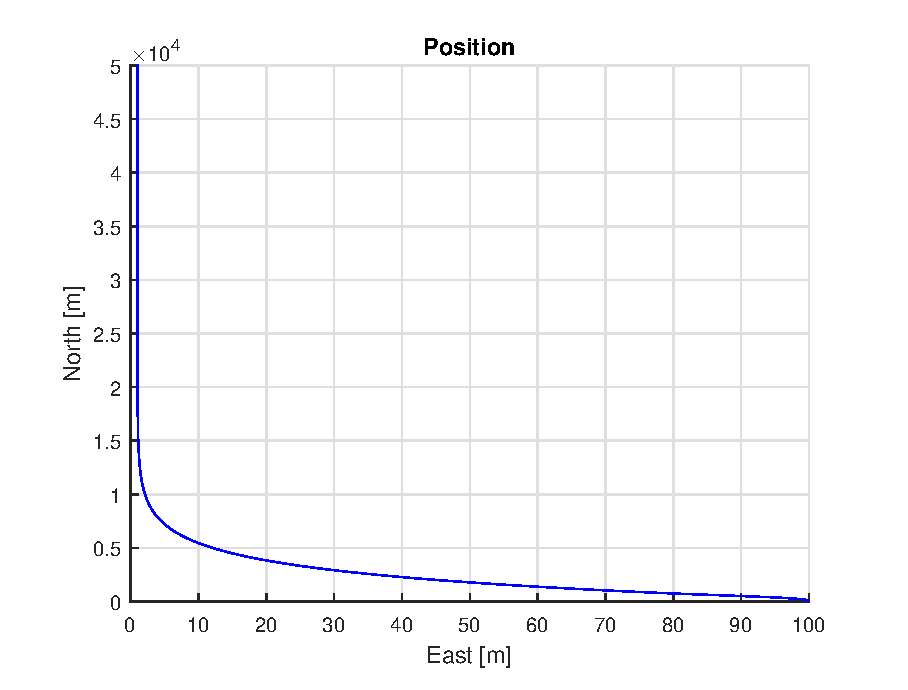
\includegraphics[width=\textwidth]{plots/2_4_pos_PD.eps}
        \caption{Position}
        \label{fig:24_pos_pd}
    \end{subfigure}
    \begin{subfigure}[b]{0.45\textwidth}
        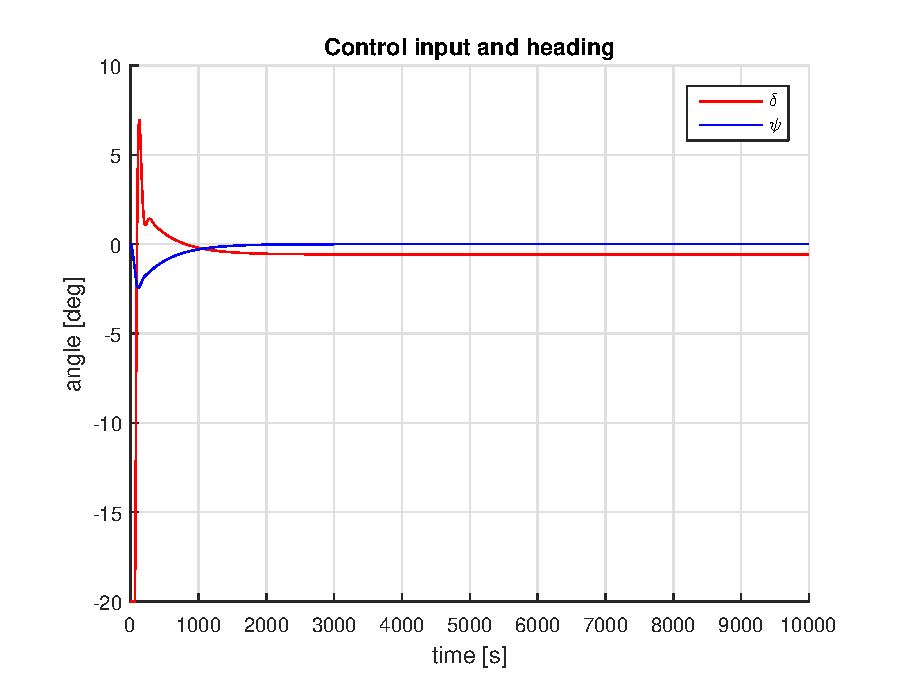
\includegraphics[width=\textwidth]{plots/2_4_ctrl_PD.eps}
        \caption{Control input and heading}
        \label{fig:24_ctrl_pd}
    \end{subfigure}
    \begin{subfigure}[b]{0.45\textwidth}
        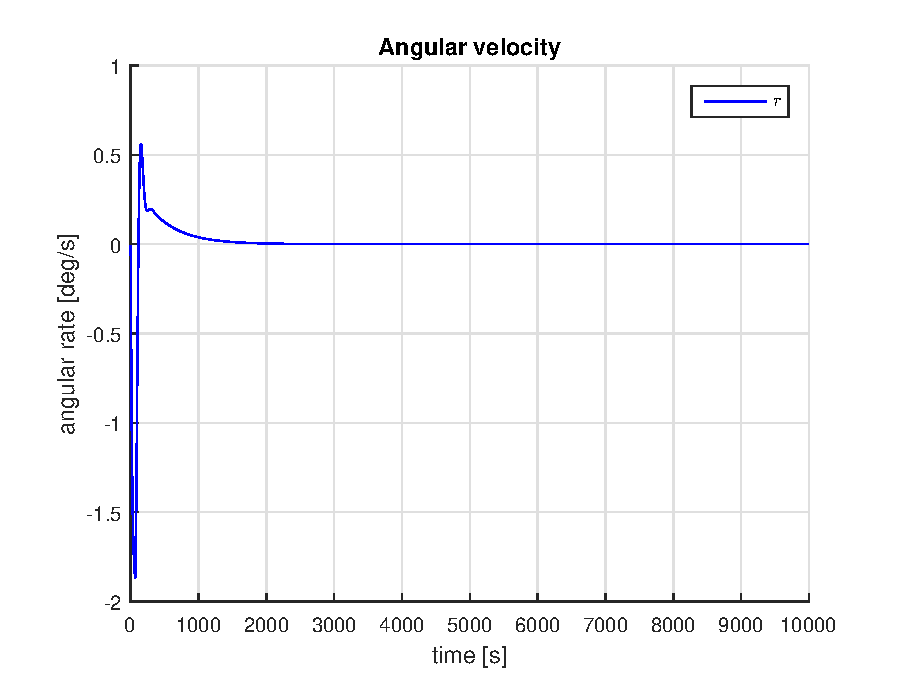
\includegraphics[width=\textwidth]{plots/2_4_r_PD.eps}
        \caption{Angular Velocity}
        \label{fig:24_r_pd}
    \end{subfigure}
    \caption{PD controller}\label{fig:24_PD}
\end{figure}

With a PD controller, we get the response as shown in Figure \ref{fig:24_PD}. We see that we get a slight stationary error due to the bias on the rudder. Introducing an integral effect in the controller to combat this, we get the results shown in Figure \ref{fig:24_PID}.

\begin{figure}[h]
    \centering
    \begin{subfigure}[b]{0.45\textwidth}
        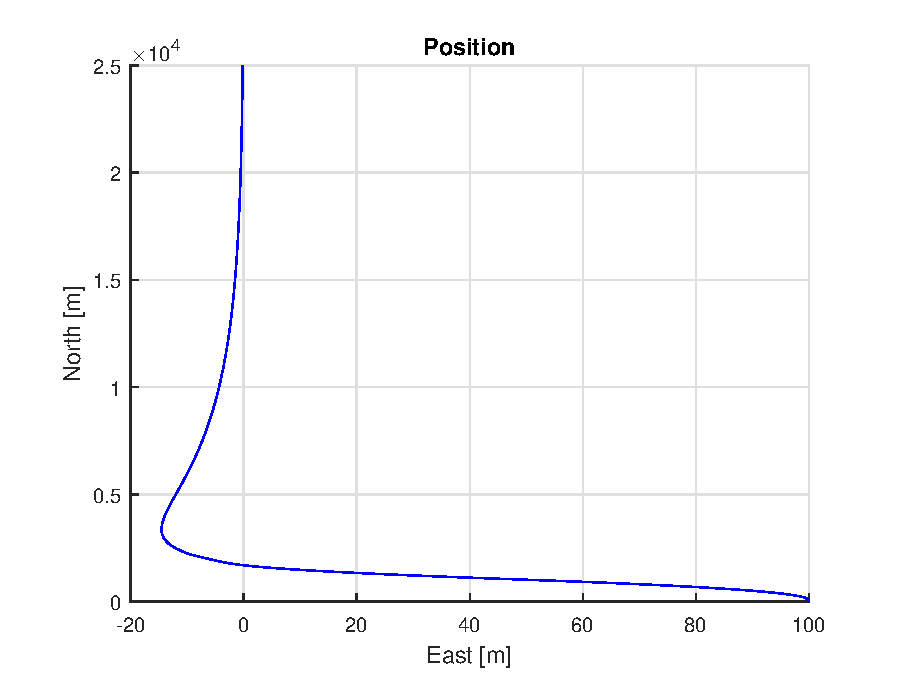
\includegraphics[width=\textwidth]{plots/2_4_pos_PID.eps}
        \caption{Position}
        \label{fig:24_pos_pid}
    \end{subfigure}
    \begin{subfigure}[b]{0.45\textwidth}
        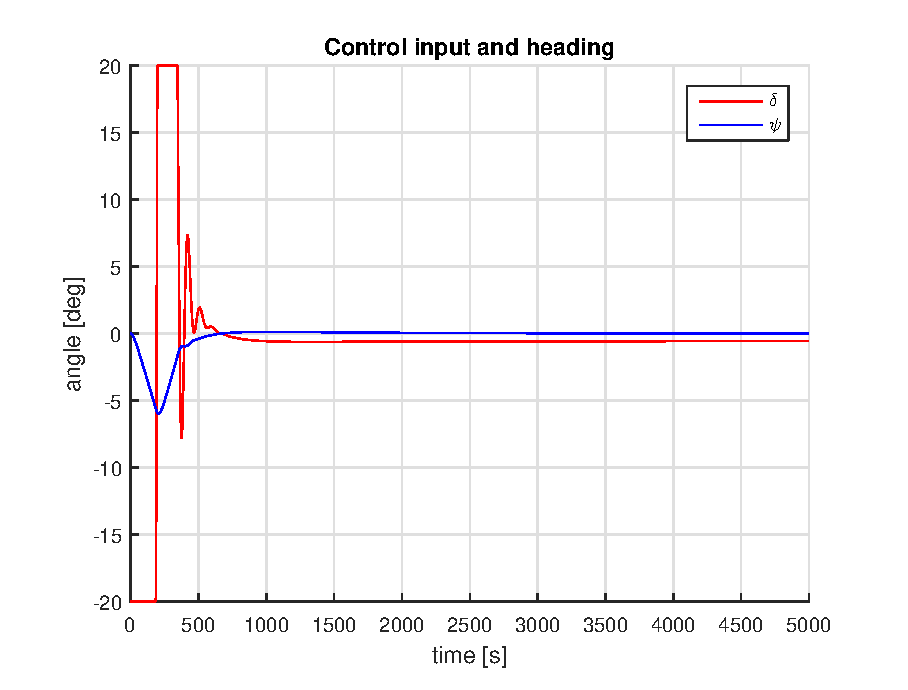
\includegraphics[width=\textwidth]{plots/2_4_ctrl_PID.eps}
        \caption{Control input and heading}
        \label{fig:24_ctrl_pid}
    \end{subfigure}
    \begin{subfigure}[b]{0.45\textwidth}
        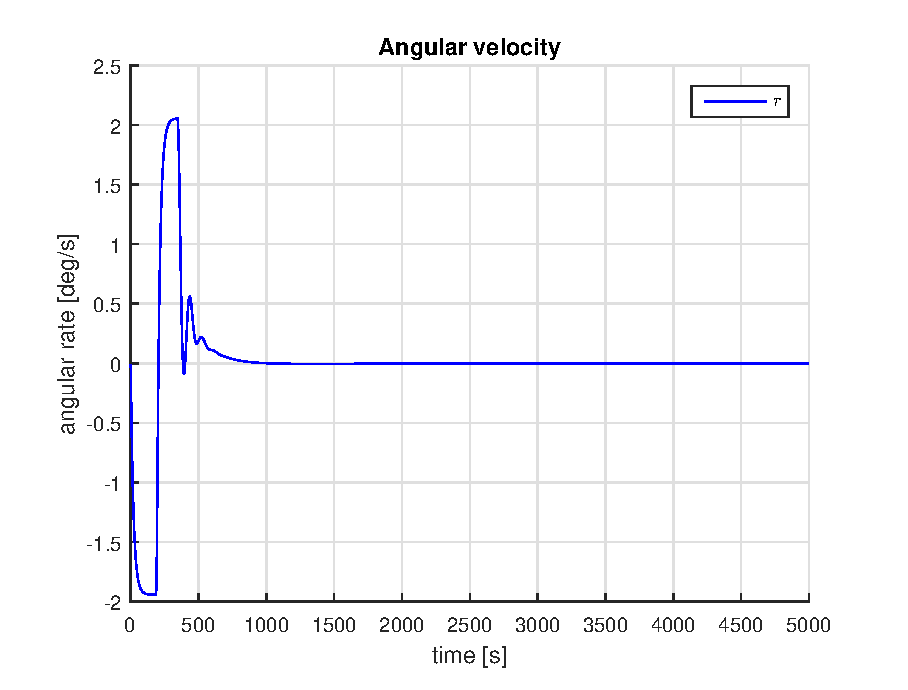
\includegraphics[width=\textwidth]{plots/2_4_r_PID.eps}
        \caption{Angular Velocity}
        \label{fig:24_r_pid}
    \end{subfigure}
    \caption{PID controller}\label{fig:24_PID}
\end{figure}

We now see that the stationary error is gone, but we now have a more complex controller to tune. We were unable to remove the overshoot while keeping the system stable. How critical this overshoot is would depend entirely on the specific use case of the system. The same is true for how aggressive the controller should be; the most efficient path to a point far ahead up north would be a straight line from the initial point. However, if it is more important to follow the path at $y=0$ at all times than to reach the destination as fast as possible, the controller should be more aggressively tuned.